% SESSION TIMELINE. Two people, one session. The wearer's exposure is the
% binding constraint, so it is drawn as its own track.
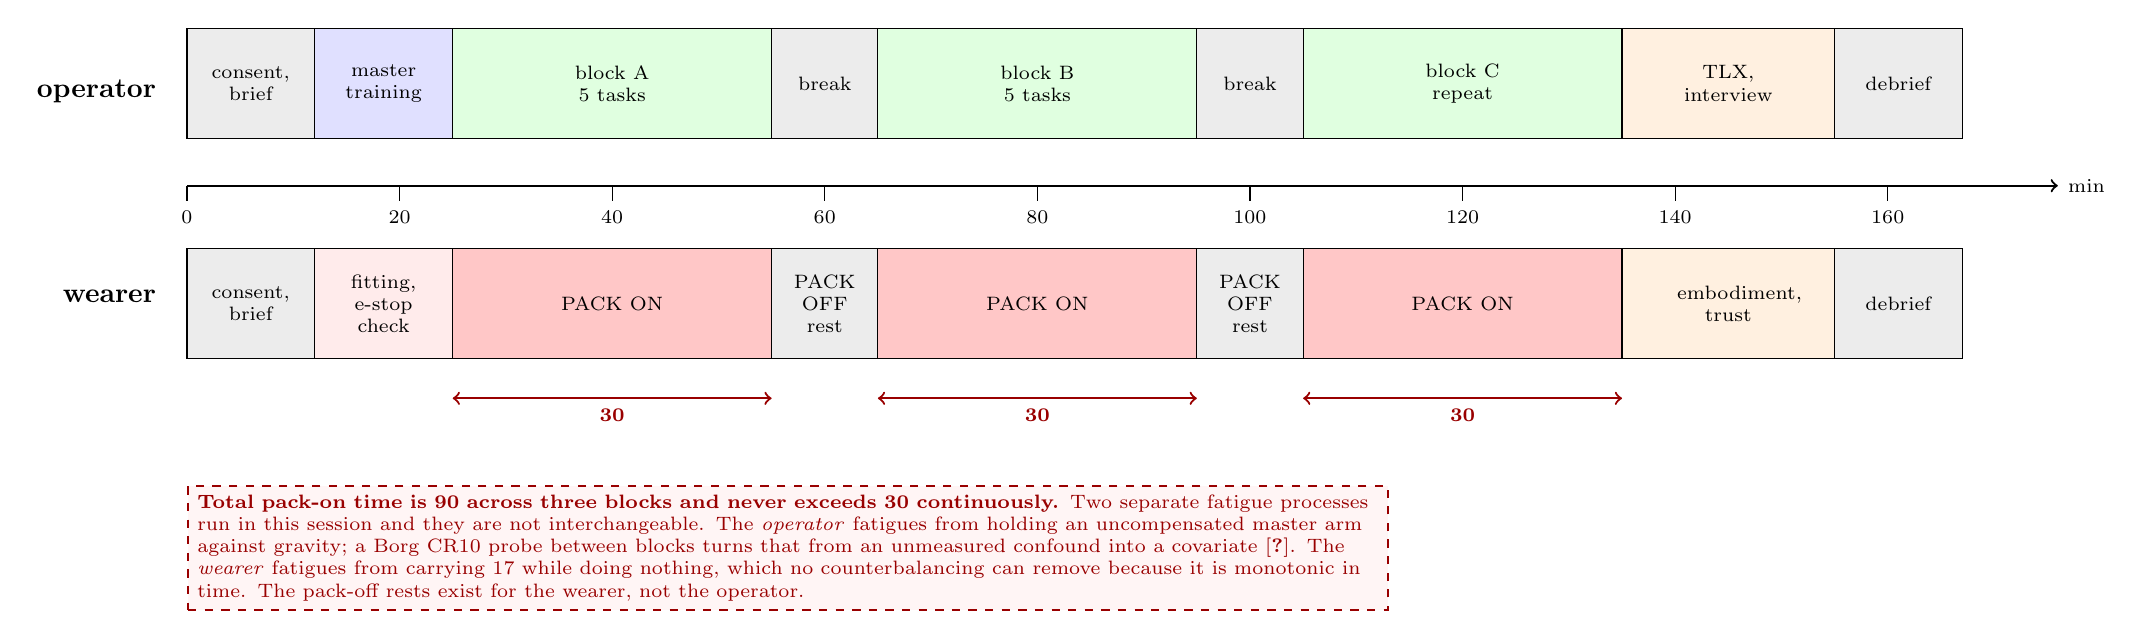
\begin{tikzpicture}[x=1.35mm, y=1mm, font=\scriptsize]

\draw[->, thick] (0,0) -- (176,0) node[right] {min};
\foreach \t in {0,20,...,160} \draw (\t,0) -- (\t,-2) node[below] {\t};

% operator track
\node[anchor=east, font=\bfseries] at (-2, 12) {operator};
\foreach \a/\b/\c/\l in {0/12/gray!15/{consent,\\brief},
                         12/25/blue!12/{master\\training},
                         25/55/green!12/{block A\\5 tasks},
                         55/65/gray!15/{break},
                         65/95/green!12/{block B\\5 tasks},
                         95/105/gray!15/{break},
                         105/135/green!12/{block C\\repeat},
                         135/155/orange!12/{TLX,\\interview},
                         155/167/gray!15/{debrief}}
{
  \pgfmathsetmacro{\m}{(\a+\b)/2}
  \draw[fill=\c] (\a,6) rectangle (\b,20);
  \node[align=center, text width=13mm] at (\m,13) {\l};
}

% wearer track
\node[anchor=east, font=\bfseries] at (-2, -14) {wearer};
\foreach \a/\b/\c/\l in {0/12/gray!15/{consent,\\brief},
                         12/25/red!8/{fitting,\\e-stop check},
                         25/55/red!22/{PACK ON},
                         55/65/gray!15/{PACK OFF\\rest},
                         65/95/red!22/{PACK ON},
                         95/105/gray!15/{PACK OFF\\rest},
                         105/135/red!22/{PACK ON},
                         135/155/orange!12/{embodiment,\\trust},
                         155/167/gray!15/{debrief}}
{
  \pgfmathsetmacro{\m}{(\a+\b)/2}
  \draw[fill=\c] (\a,-22) rectangle (\b,-8);
  \node[align=center, text width=13mm] at (\m,-15) {\l};
}

\draw[<->, thick, red!60!black] (25,-27) -- (55,-27)
   node[midway, below, font=\scriptsize\bfseries, red!60!black] {\SI{30}{\minute}};
\draw[<->, thick, red!60!black] (65,-27) -- (95,-27)
   node[midway, below, font=\scriptsize\bfseries, red!60!black] {\SI{30}{\minute}};
\draw[<->, thick, red!60!black] (105,-27) -- (135,-27)
   node[midway, below, font=\scriptsize\bfseries, red!60!black] {\SI{30}{\minute}};

\node[draw, dashed, thick, red!60!black, fill=red!4, text width=150mm,
      align=left, anchor=west] at (0, -46)
  {\textbf{\color{red!60!black}Total pack-on time is \SI{90}{\minute} across
   three blocks and never exceeds \SI{30}{\minute} continuously.} Two separate
   fatigue processes run in this session and they are not interchangeable. The
   \emph{operator} fatigues from holding an uncompensated master arm against
   gravity; a Borg CR10 probe between blocks turns that from an unmeasured
   confound into a covariate \cite{borg1982perceived}. The \emph{wearer}
   fatigues from carrying \SI{17}{\kilo\gram} while doing nothing, which no
   counterbalancing can remove because it is monotonic in time. The pack-off
   rests exist for the wearer, not the operator.};
\end{tikzpicture}
